\setchapterpreamble[u]{\margintoc}
\chapter{Introduction}
\labch{intro}

\section{The Main Ideas}

This is some text and a link to 
\href{https://bradflaugher.com}{bradflaugher.com}.  
\sidenote{Snarky sidenote!} 

\section{What This Class Does}
\labsec{does}

(see also \vrefsec{intro}) 

\begin{description}
	\item[List Item 1] It's a list, yo!
	\item[List Item 2] Second item in the list.
\end{description}

\begin{marginfigure}[-5.5cm]
	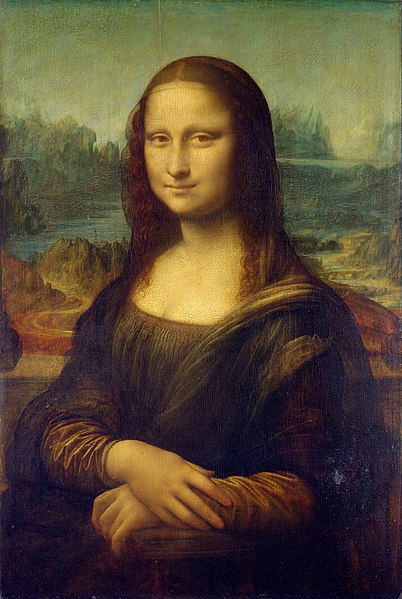
\includegraphics{monalisa}
	\caption[The Mona Lisa]{The Mona Lisa.\\ 
	\url{https://commons.wikimedia.org/wiki/File:Mona_Lisa,_by_Leonardo_da_Vinci,_from_C2RMF_retouched.jpg}}
	\labfig{marginmonalisa}
\end{marginfigure}


\begin{lstlisting}[style=kaolstplain,linewidth=1.5\textwidth]
cd myproject
docker run tensorflow
#profit!
\end{lstlisting}

\url{tex.stackexchange.org} for help.
